\ylDisplay{Küttekeha} % Ülesande nimi
{Mihkel Heidelberg} % Autor
{lõppvoor} % Voor
{2007} % Aasta
{G 7} % Ülesande nr.
{6} % Raskustase
{
% Teema: Termodünaamika
\ifStatement
Teatud ruumi köetakse sellise küttekehaga, mille võimsus $P$ sõltub ruumi temperatuurist nagu on näidatud joonisel. Kui välistemperatuur on $T_1$, siis ruumi temperatuur stabiliseerub $T_2$ juures (need temperatuurid on märgitud graafikul). Millise temperatuurini tõuseb toatemperatuur, kui välistemperatuur tõuseb $T_3$-ni (leida see temperatuur graafilise konstrueerimise abil). Soojusvahetus keskkonnaga on võrdeline temperatuuride vahega.

\begin{center}
	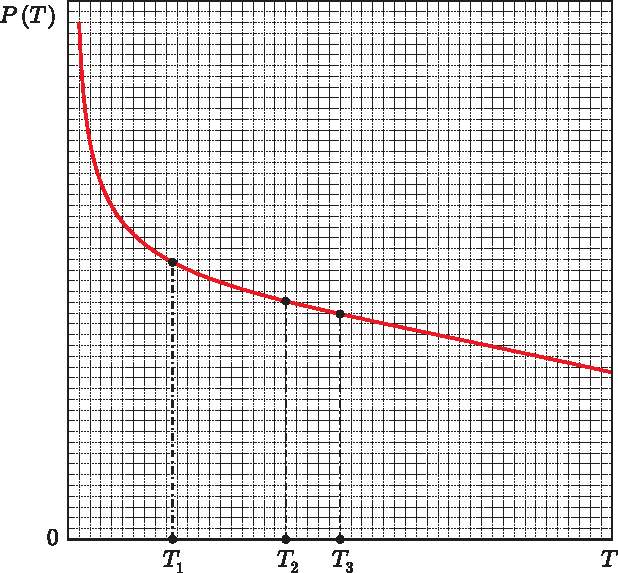
\includegraphics[width=0.8\linewidth]{2007-v3g-07-yl}
\end{center}
\fi


\ifHint
Tasakaalulises olukorras on ruumist eemalduv soojuse hulk võrdne küttekeha poolt toodetud soojusega. Selle põhjal saab leida esialgsest olukorrast keskkonna ja ruumi vahelise soojusvahetuse võrdelisusteguri ning saadud tulemust kasutada pärastise tasakaalulise temperatuuri leidmiseks.
\fi


\ifSolution
Et ruumist eemalduva soojuse hulk on stabiilses olukorras võrdne küttekeha poolttoodetud soojusega, siis $P(T_2) = k(T_2 - T_1)$, $k = \frac{P(T_2)}{T_2-T_1}$. Teisel juhul jääb $k$ samaks:
\[
P(T_4) = \frac{P(T_2)}{T_2-T_1} (T_4 - T_3), 
\]
kust on näha, et punkt ($T_4$, $P(T_4)$) peab asetsema sirgel, mis läbib punkti ($T_3$, $0$) ja on sama tõusuga ($k$), kui punkte ($T_2$, $P(T_2)$) ja ($T_1$, $0$) ühendav sirge. Joonistades sellise sirge, saame graafikute lõikepunktist vastuse. 
\fi
}